\section{Introducci\'on}

En este segundo trabajo, el objetivo es brindar otras vistas sobre lo realizado en el trabajo anterior con respecto a la cadena Mes\%. Para ello utilizamos las siguientes técnicas: 

\begin{itemize}
\item \textbf{Diagrama de casos de uso}: Este diagrama permite mostrar las interacciones de los actores que participan en alguna operación del sistema. También detallar quién realiza cada operación y observar los estereotipos “incluye” y “extiende” entre casos de uso.
\item \textbf{Diagrama de clases}: Este diagrama permite observar los conceptos más importantes en un sistema, que los llamaremos clases. También permite observar los atributos de las clases, relaciones de herencia, clases de asociación y relaciones entre clases.
\item \textbf{Diagrama de estados}: Este diagrama permite observar el comportamiento de los distintos componentes. Solo se modela los componentes que necesitan sincronizarse con otros.
\item \textbf{Diagramas de actividad}: En este diagrama se pueden observar las operaciones necesarias para realizar alguna tarea en el sistema. Estas tienen asociadas un orden y pueden realizarse en forma paralela. También se pueden observar andariveles, que son los responsables de cumplir dicha operación.
\end{itemize}



Para realizar todo este análisis, partimos de uno de los diagramas de contexto \textit{(el número 3)} presentados en el trabajo anterior. Dicho diagrama sufrió algunas modificaciones a medida que fuimos realizando este nuevo trabajo ya que notamos ciertas falencias en el mismo. A continuación presentamos el diagrama de contexto elegido, señalando en color rojo las modificaciones realizadas:

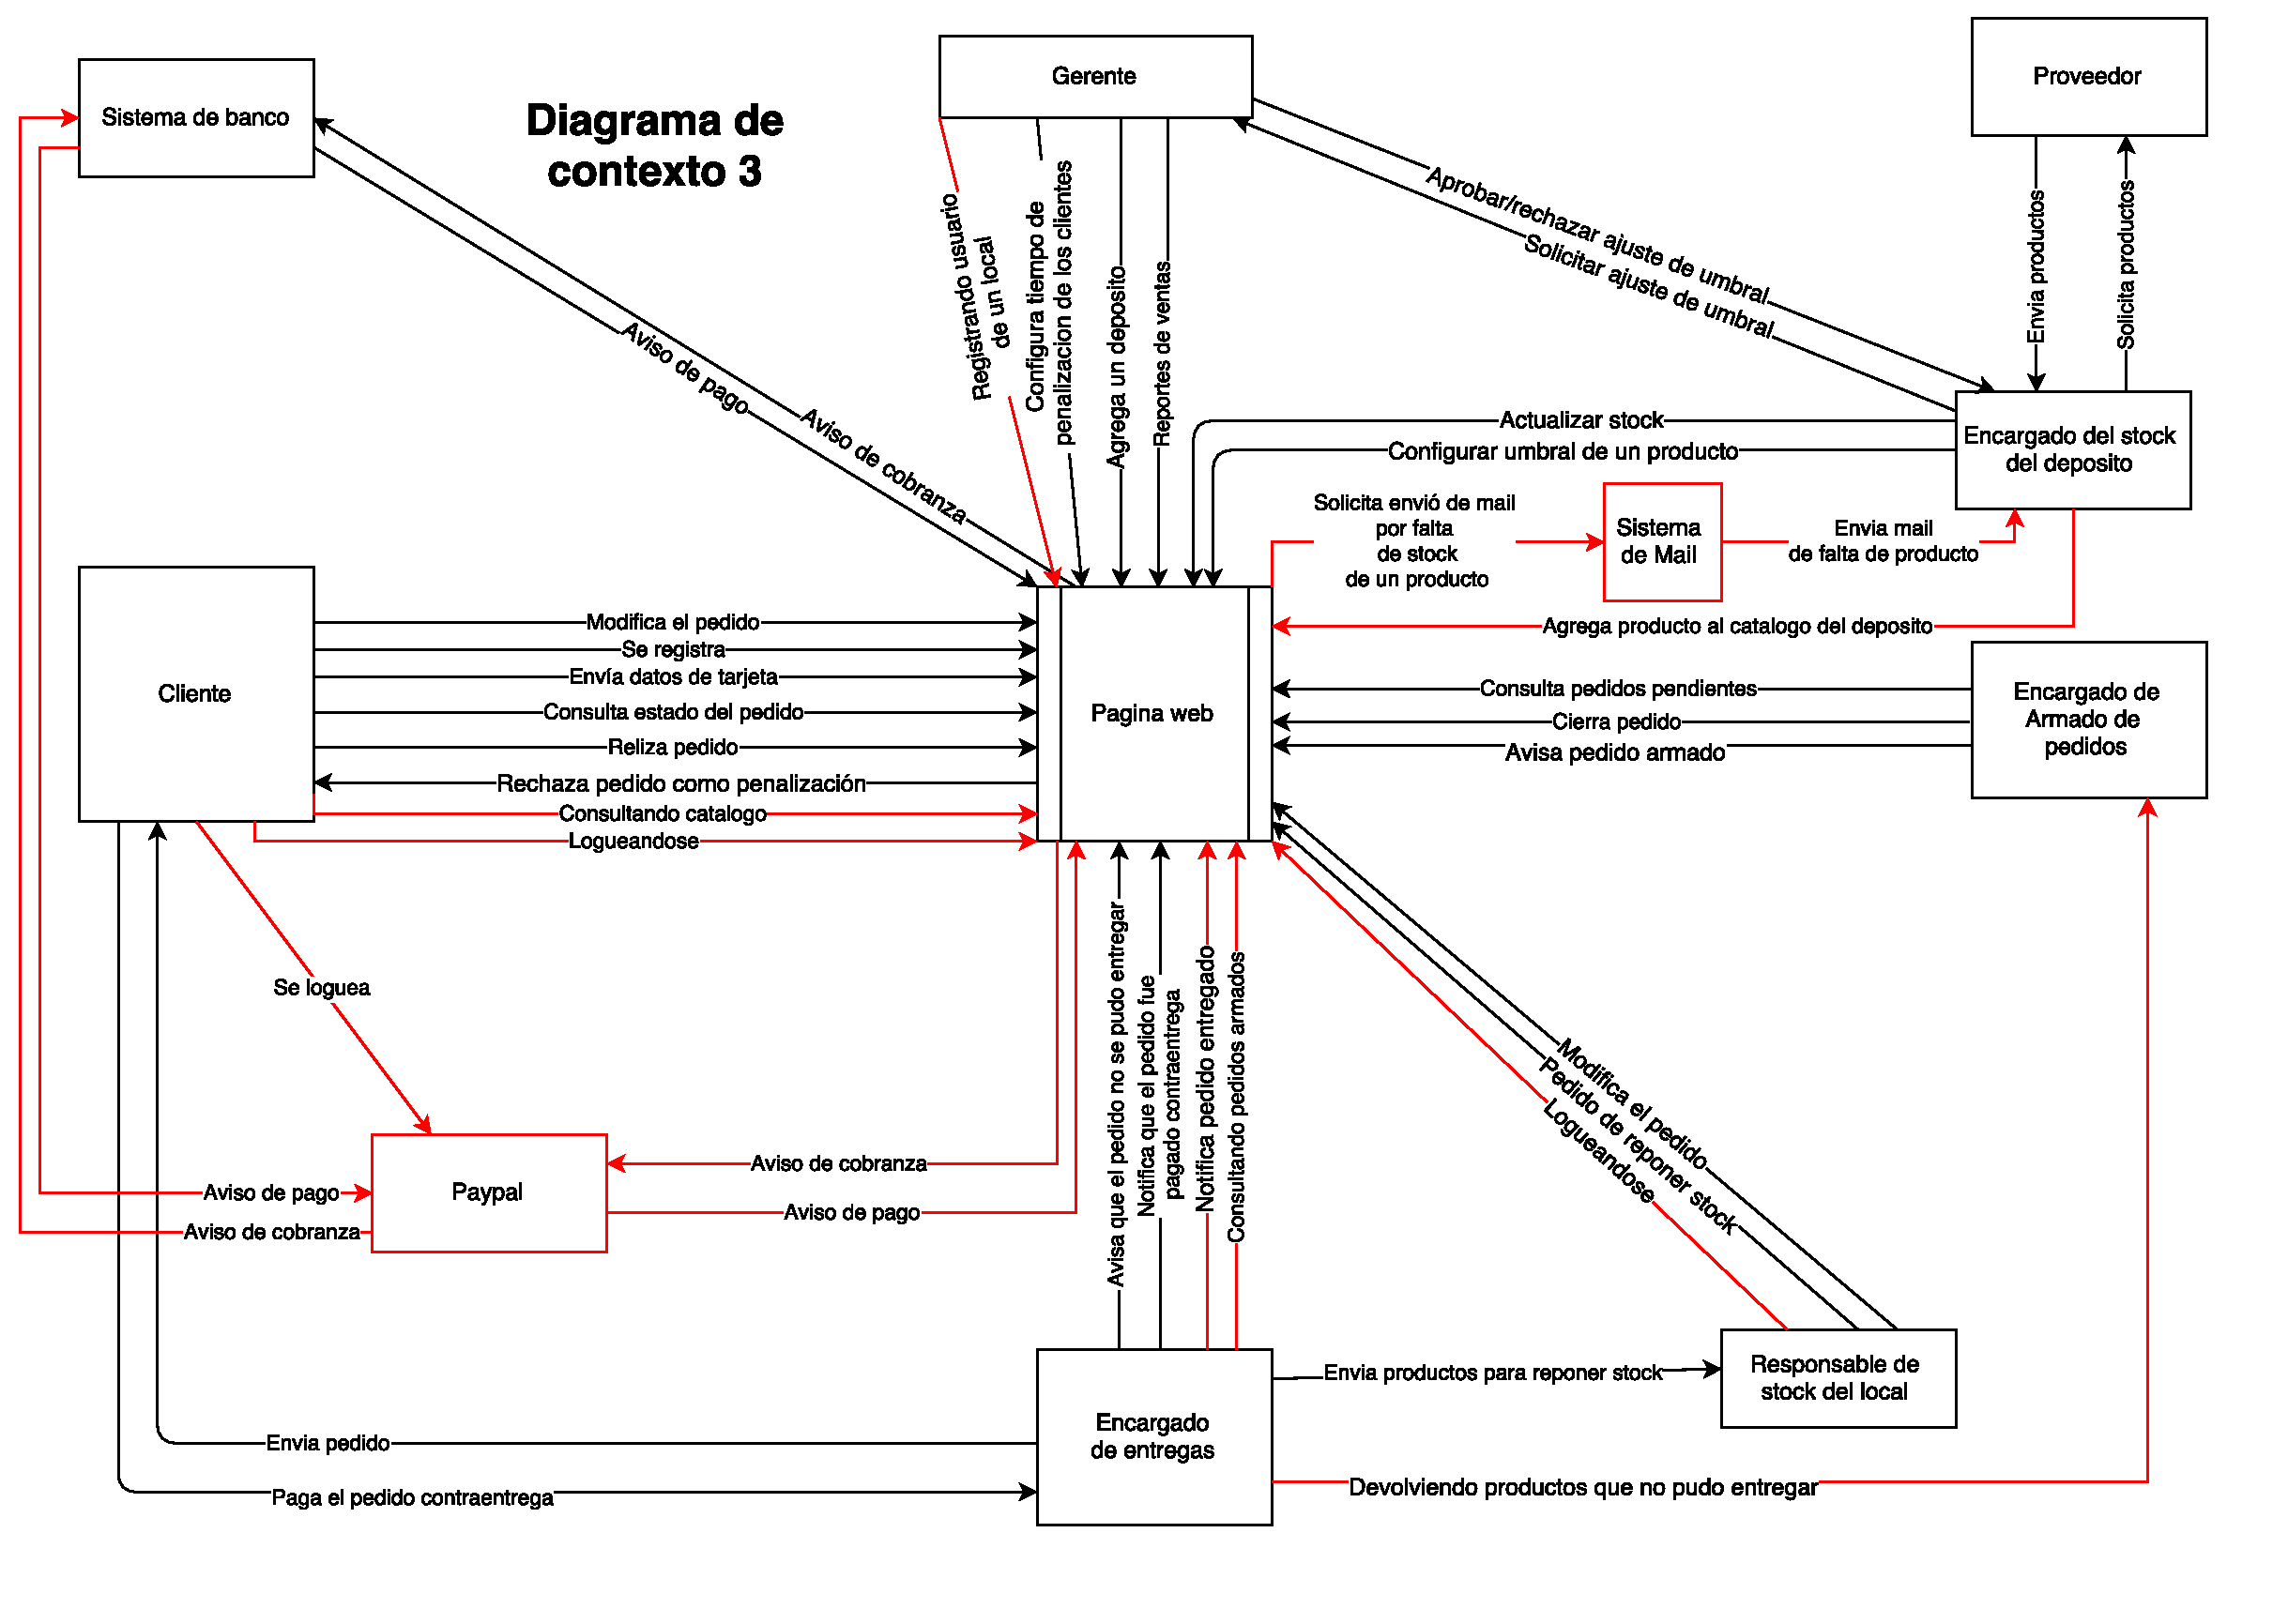
\includegraphics[scale=0.5, angle=90]{secciones/diagramaContexto}